\documentclass[../main]{subfiles}

\begin{document}
\section{Hoja de ruta}

\subsection{Configuración de Hardware}

\setcounter{subsubsection}{-1}

\subsubsection{Recursos a usar}

\begin{itemize}
	\item ESP32: Controlador principal con conectividad Wi-Fi.
	\item Sensor BME280: Sensor para medir temperatura, humedad y presión.
	\item Sensor MQ135: Sensor para la detección de la concentración de CO2 en el aire.
	\item Sensor de Humedad de Suelo: Sensor analógico para medir el nivel de humedad del suelo.
	\item Protoboard y Jumpers: Para facilitar las conexiones de prueba.
	\item Fuente de Alimentación: Batería o adaptador USB de 5V.
	\item Cables Dupont: Para realizar las conexiones entre los sensores y el ESP32.
\end{itemize}

\subsubsection{Diagrama de Conexiones}

\begin{itemize}
	\item ESP32: Este será el controlador principal y estará encargado de leer los datos de cada sensor.
	\item BME280: Este sensor utiliza la comunicación I2C para conectarse con el ESP32. Las conexiones necesarias son:
	      \begin{enumerate}
		      \item VCC a \qty{3.3}{\V} del ESP32.
		      \item GND a GND del ESP32.
		      \item SCL al pin D22 del ESP32.
		      \item SDA al pin D21 del ESP32.
	      \end{enumerate}
	\item MQ135: Para el sensor MQ135, se utilizará la salida analógica para la detección de CO2.
	      \begin{enumerate}
		      \item VCC a \qty{5}{\V} del ESP32.
		      \item GND a GND del ESP32.
		      \item AOUT a un pin analógico del ESP32.
	      \end{enumerate}
	\item Sensor de Humedad de Suelo: El sensor de humedad de suelo puede ser analógico o digital. Se optará por la salida analógica para una medición más precisa.
	      \begin{enumerate}
		      \item VCC a \qty{3.3}{\V} del ESP32.
		      \item GND a GND del ESP32.
		      \item AOUT a un pin analógico del ESP32.
	      \end{enumerate}
\end{itemize}

\subsubsection{Soporte del ESP32 en Arduino IDE}

Para poder programar en ESP32 con Arduino, es necesario agregar un URL en el
gestor de placas lo siguiente:
\url{https://dl.espressif.com/dl/package_esp32_index.json}

\begin{figure}[H]
	\centering
	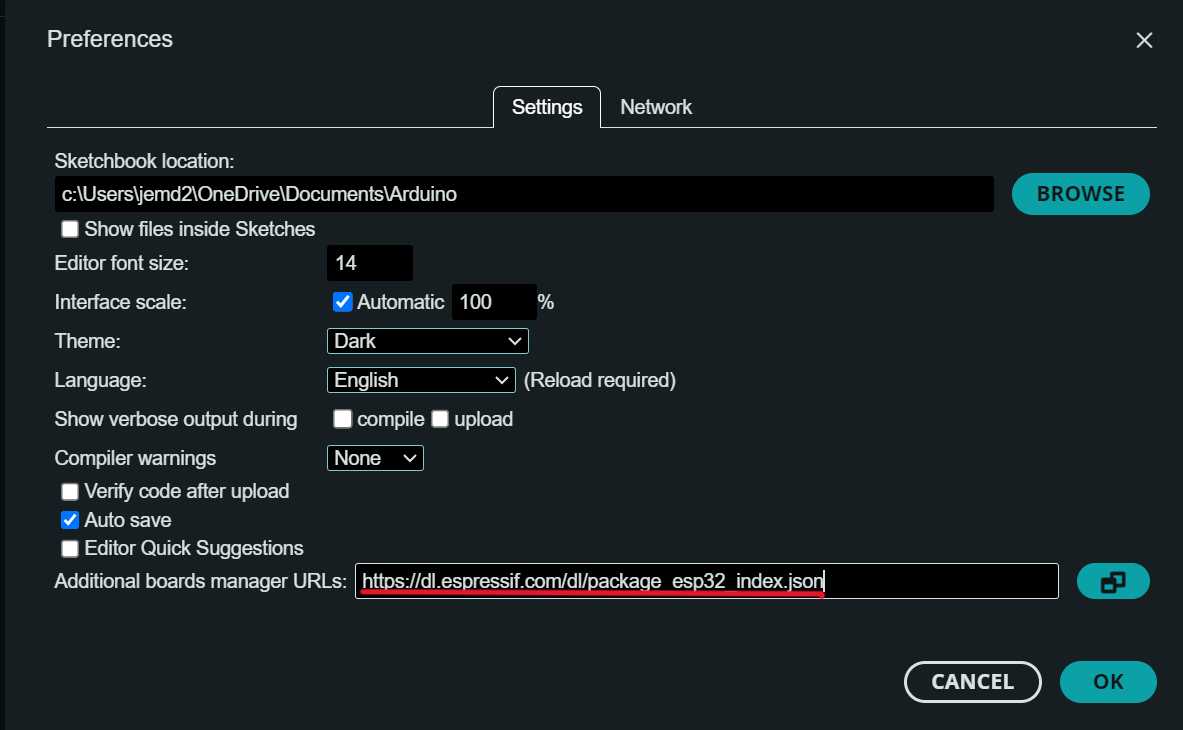
\includegraphics[width = 13cm]{res/configuracionParaEsp32.png}
\end{figure}

\subsubsection{Conexión con Firebase}

Para realizar una conexión a Firebase desde tu ESP32, es utilizada la biblioteca
Firebase ESP32 Client.

\subsection{Programación de aplicación}

\setcounter{subsubsection}{-1}

\subsubsection{Recursos a usar}

\begin{itemize}
	\item Kotlin: lenguaje principal de desarrollo
	      \footnote{\url{https://kotlinlang.org/}}
	\item Firebase Realtime Database: almacenamiento de observaciones y perfiles
	      \footnote{\url{https://firebase.google.com/}}
	\item Androidplot: biblioteca para la creación de gráficos
	      \footnote{\url{https://github.com/halfhp/androidplot}}
\end{itemize}


\begin{figure}[H]
	\centering
	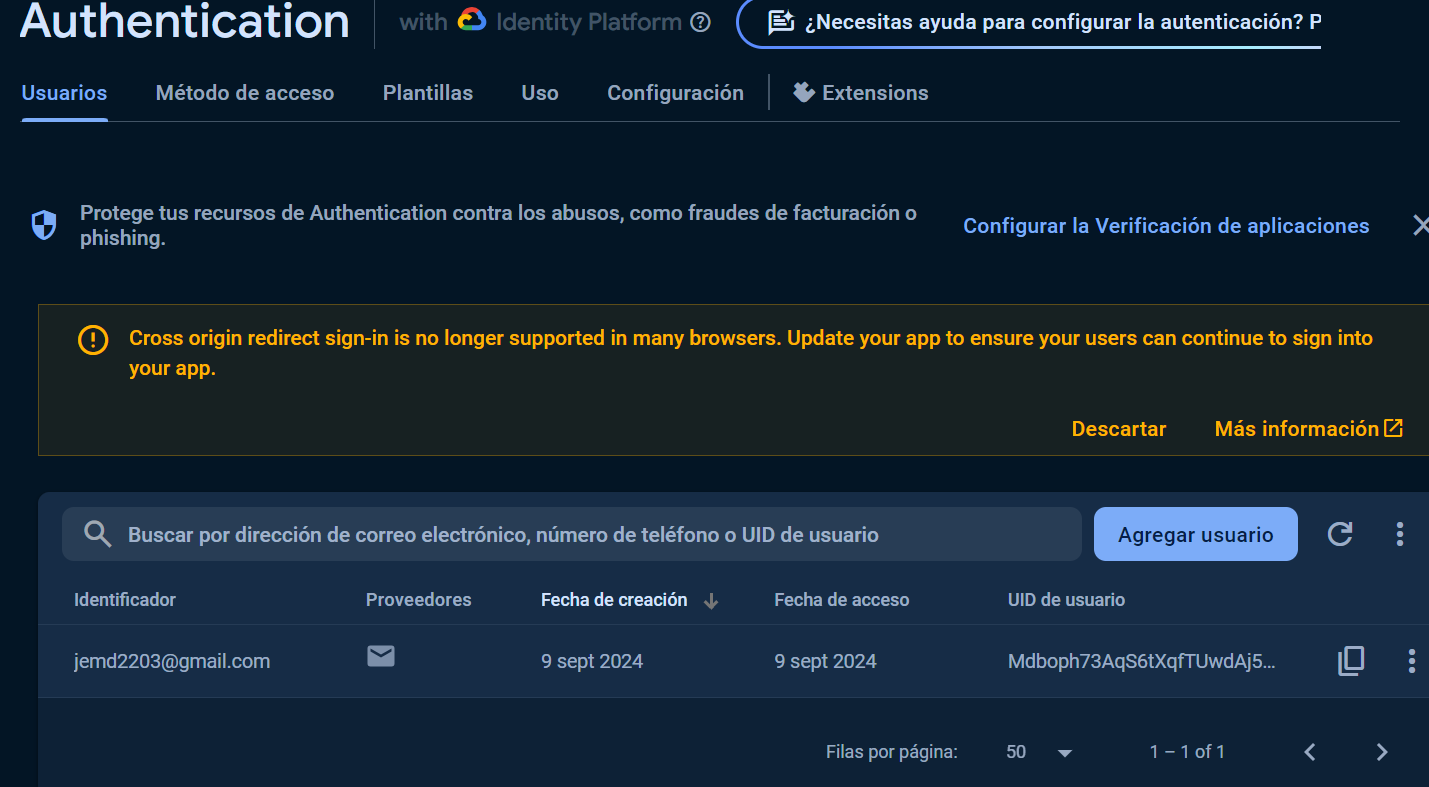
\includegraphics[width=15cm]{res/AutenticacionFireBase.png}
	\caption{Usuario registrado en Firebase}
	\label{FiguraDeAutenticacion}
\end{figure}

\subsubsection{Visualización de datos y gráficos}

\begin{itemize}
	\item Parámetros ambientales:
	      Los valores de temperatura, humedad, presión y concentración de \ce{CO2}
	      aparecerán en la pantalla principal junto a indicadores de su
	      adecuación al perfil de monitoreo
	\item Generación de gráficos:
	      La aplicación permitirá también la visualización gráfica de los datos
	      históricos. Para implementar esta funcionalidad, se usará la biblioteca
	      AndroidPlot que facilita la creación de gráficos de líneas, gráficos de
	      barras y otras representaciones visuales.
	\item Datos históricos:
	      Los usuarios podrán acceder a un historial de las condiciones ambientales
	      registradas, lo cual será útil para la toma de decisiones relacionadas
	      con el cultivo.
\end{itemize}

\begin{figure}[H]
	\centering
	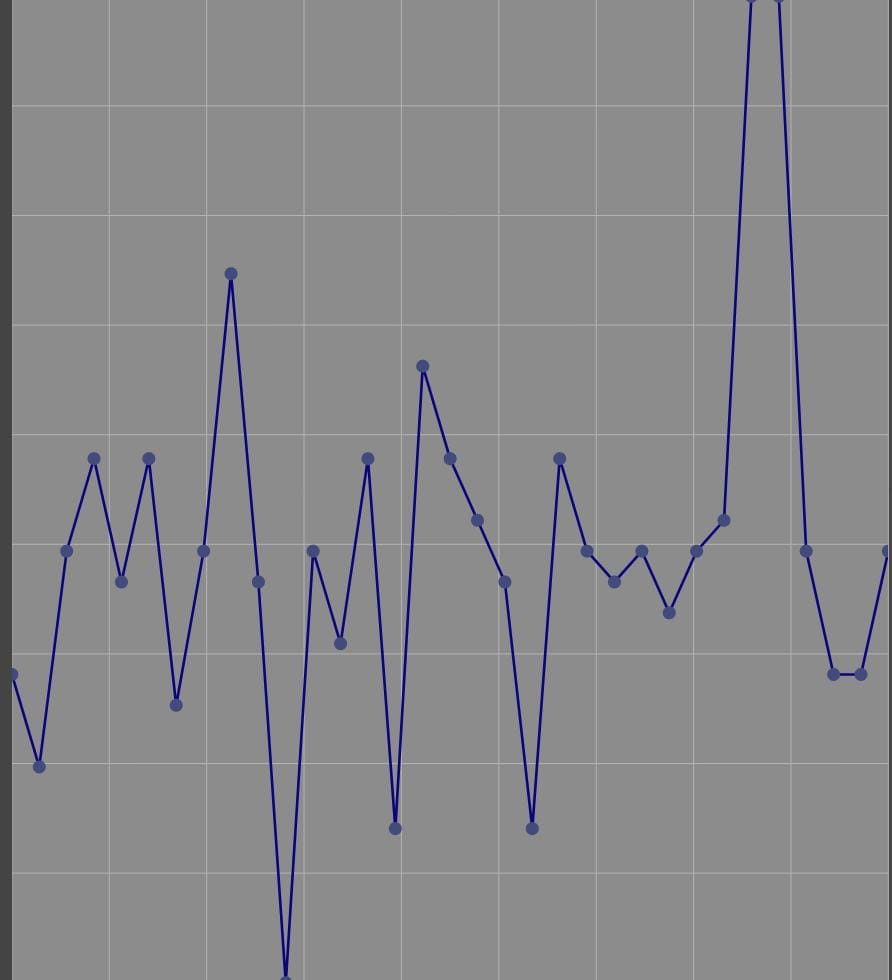
\includegraphics[width=10cm]{res/GráficosParaAplicación.jpeg}
	\caption{Gráficos generado por biblioteca}
	\label{FiguraDeGráficos}
\end{figure}
\end{document}
